% Resultate
\section{Resultate}

\subsection{Bekannte Fehler}

\subsubsection{iOS - Add to homescreen}
Eine sehr nützliche Funktionalität, welche Apple im Mobile Safari-Browser anbietet ist die \emph{Add to homescreen}-Funktion.

\begin{figure}[H]
\subfigure{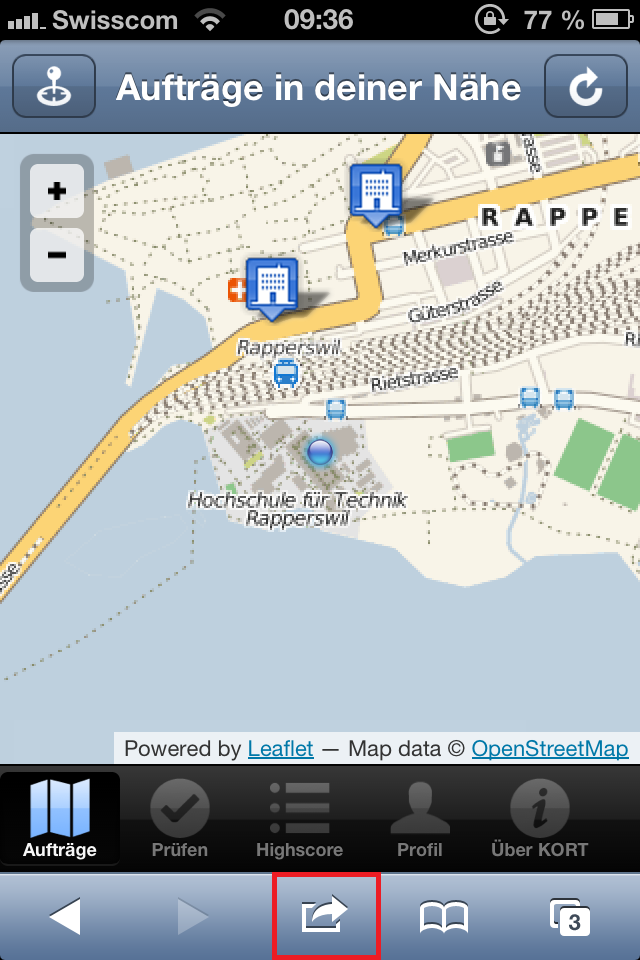
\includegraphics[width=0.23\textwidth]{images/bugs/kort-add_to_homescreen_1}}
\hfill
\subfigure{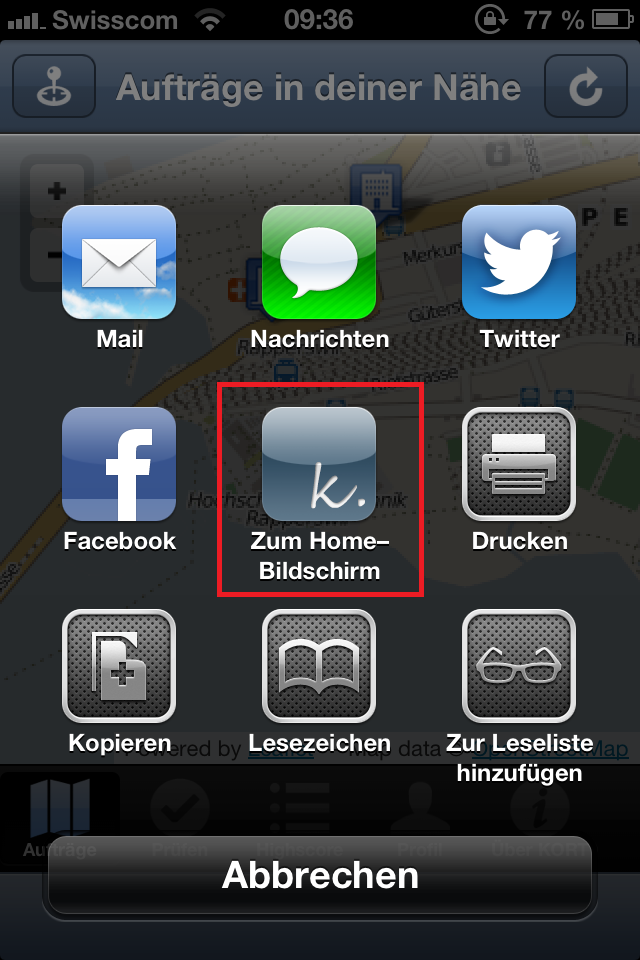
\includegraphics[width=0.23\textwidth]{images/bugs/kort-add_to_homescreen_2}}
\hfill
\subfigure{
\includegraphics[width=0.23\textwidth]{images/bugs/kort-add_to_homescreen_3}}
\hfill
\subfigure{
\includegraphics[width=0.23\textwidth]{images/bugs/kort-add_to_homescreen_4}}
\caption{iOS - "`Add to homescreen"'-Funktion}
\end{figure}

Dadurch wird ein App-ähnlicher Bookmark der aktuellen Webseite auf dem Homescreen erstellt.
Dieser erhält ein hinterlegtes Icon und einen Titel.
Beim Starten der App erscheint ein Splashscreen, welchen man ebenfalls in der Webseite definieren kann. Zudem öffnet sich der Browser ohne jegliche Toolbars wie der Adressleiste oder der Navigationsbar.

Leider hat die verwendete Version (2.1.0) des Sencha Touch Frameworks Fehler bei der Anzeige von einigen GUI-Komponenten.
So werden in unserem Fall nach dem Splashscreen lediglich ein weisser Bildschirm angezeigt.

\subsubsection{App Build}
Wie in Abschnitt \ref{sencha-cmd} beschrieben, basiert die App vollständig auf dem Sencha-eigenen Build-Tool \emph{Sencha Cmd 3.0.0.250}. Darin sind aber noch einige Bugs vorhanden.

Bei \textsc{Kort} besteht dabei ein Problem bei der fest eingebauten Komprimierung der JavaScript-Sourcen.
Während diesem Prozess werden lokale Variablennamen mit einzelnen Buchstaben abgekürzt.
Dabei treten Konflikte mit der Leaflet-Library auf, welche den Buchstaben \emph{L} als Namespace verwendet.

\textbf{Workaround}

Um diese Problem zu umgehen, mussten wir das Build-Skript von Sencha Cmd minimal anpassen.
So mussten wir die Zeile, welche den \gls{Microloader} komprimiert auskommentieren (siehe Code-Ausschnitt \ref{senchacmd-workaround}).
Diese befindet sich in folgender Datei:

\inlinecode{/<Sencha Cmd Verzeichnis>/plugins/touch/current/app-build.js}

\inlinecode{Zeile 362: //content = compressor.compress(content);}

\lstset{language=JavaScript}
\begin{lstlisting}[float, caption=Sencha Cmd Workaround, label=senchacmd-workaround]
processIndex = function () {
	[...]
	
	compressor = new ClosureCompressor();
	microloader = (environment == 'production'
		? 'production'
		: 'testing') +
		'.js';
	_logger.debug("using microloader : {}", microloader);
	content = readFileContent(joinPath(sdk, "microloader", microloader));
	//content = compressor.compress(content);
	remotes = [
		'<script type="text/javascript">' +
			content + ';Ext.blink(' +
			(environment == 'production' ? jsonEncode({
				id:config.id
			}) : appJson) + ')' +
			'</script>'
	];
	
	[...]
};
\end{lstlisting}